\documentclass{beamer}

% Language and especial characteres
\usepackage[utf8]{inputenc}
\usepackage[T1]{fontenc}
\usepackage[brazilian]{babel}

% figure
\usepackage{subfigure}
\usepackage{caption}

\usetheme{metropolis} % Use metropolis theme
\title{}

\date{03 de Dezembro de 2020}

\author{Leonardo Cardoso Botelho \\ Rafael Lima}
\institute{Universidade de Brasília}
\begin{document}
\maketitle
\begin{frame}{Sumário}
\tableofcontents
\end{frame}

\section{Controle de posição de um motor DC}
%\section{Metodologia}
\subsection{Objetivos}

% Bloco para representação de um slide
\begin{frame}{Slide de Exemplo} % título "Slide de Exemplo"

% Caixa para destaque sem titulo
\begin{block}{}
Caixa para destaque sem título
\end{block}

% Caixa para destaque sem titulo
\begin{block}{Titulo da Caixa}
Caixa para destaque com título
\end{block}

\end{frame}

\begin{frame}{Desempenho de um Sistema de Controle}
\begin{figure}
    \centering
    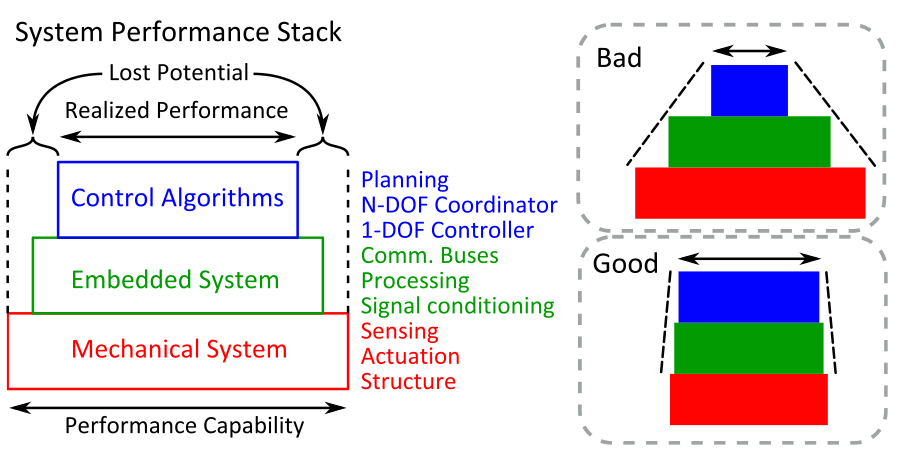
\includegraphics[width = 0.9\linewidth]{src/tex/img/system_perfomance.png}
    \caption{Representação da Capacidade de Desempenho \cite{paine2014high}}
    \label{fig:system_perfomance}
\end{figure}
\end{frame}

\section{Construção Sistema}

\subsection{Implementação em Hardware}

\begin{frame}{Planta Simulada}
\begin{figure}
    \centering
    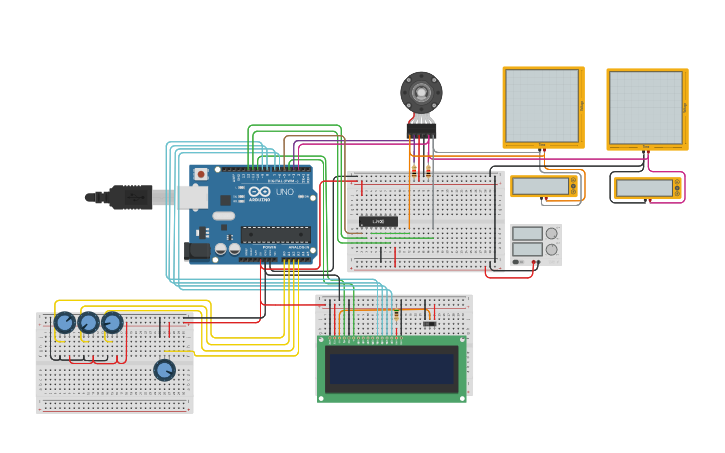
\includegraphics[width = \linewidth]{src/tex/img/pid_tinkercad.png}
    \caption{Planta no Tinkercad}
    \label{fig:control_1}
\end{figure}
\end{frame}

\begin{frame}{Planta Real}
\begin{figure}
    \centering
    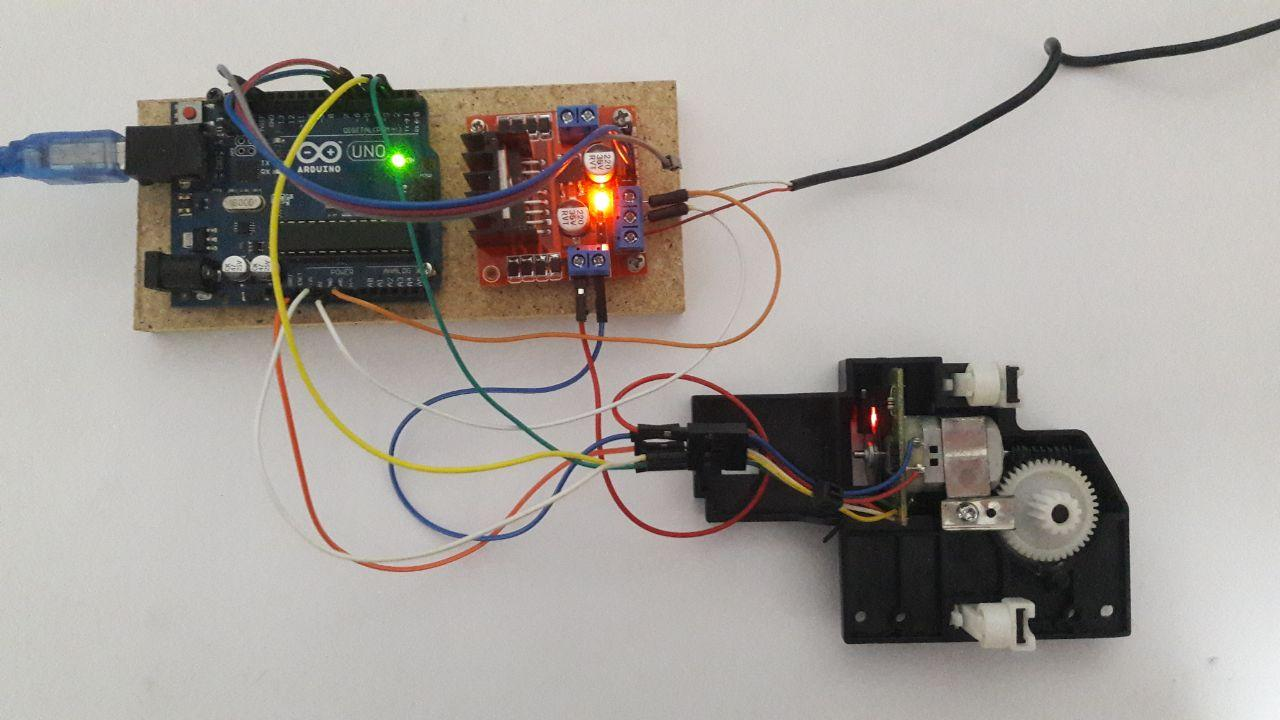
\includegraphics[width = \linewidth]{src/tex/img/full_system.jpg}
    \caption{Sistema Real}
    \label{fig:control_1}
\end{figure}
\end{frame}

\subsection{Caracterização sistema}

\begin{frame}{Identificação de Zona Morta}
\begin{figure}
    \centering
    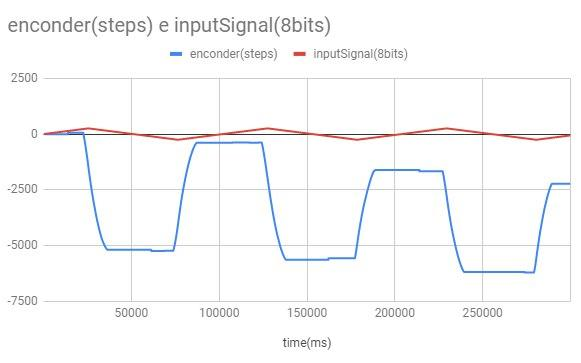
\includegraphics[width = \linewidth]{src/tex/img/grafico_dente_serra.jpg}
    \caption{Resposta um sinal triangular}
    \label{fig:control_1}
\end{figure}
\end{frame}

\begin{frame}{Modelo Sistema}
    % TODO Colocar diagrama de blocos planta em malha aberta
    \begin{block}{Transformada Z}
        \begin{equation}
        G(z) = \frac{Y(z)}{U(z)} = \beta K_e \ \alpha \frac{\left(e^{-\frac{T}{\alpha} + \frac{T^2}{\alpha}}\right)z + \left(e^{-\frac{T}{\alpha}}+e^{-\frac{T}{\alpha}}\frac{T^2}{\alpha}+1\right)  }{\left(z-1\right)\left(z-e^{-\frac{T}{\alpha}}\right)}
        \label{transfdisc}
        \end{equation}
    \end{block}
\end{frame}

\begin{frame}{Identificação do sistema}
\begin{figure}
    \centering
    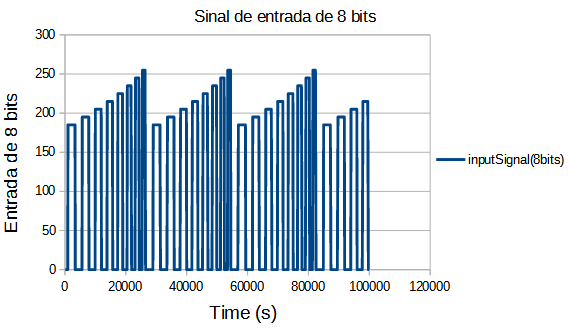
\includegraphics[width = 0.6\linewidth]{sinal_8_bits.PNG}
    \label{fig:control_1}
\end{figure}
\begin{figure}
    \centering
    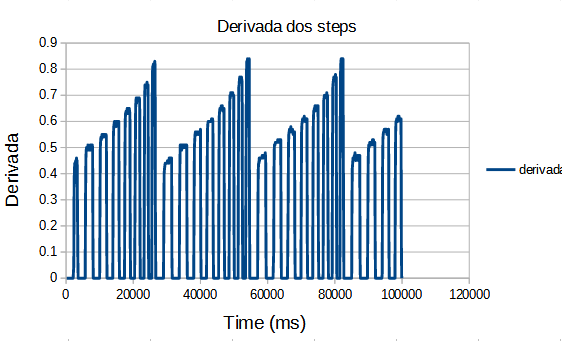
\includegraphics[width = 0.6\linewidth]{derivada_steps.PNG}
    \label{fig:control_1}
\end{figure}
\end{frame}

\begin{frame}{Função de Transferência}
    \begin{block}{Forma Geral a partir do modelo}
        \begin{equation}\label{eq:gz_general}
            G(z) = \frac{Y(z)}{U(z)} = \frac{\beta_1 z + \beta_2}{z^2 + \alpha_1 z + \alpha_2}
        \end{equation}
    \end{block}
    
    \begin{block}{Resultado Experimental}
        \begin{equation}
        G(z) = \frac{Y(z)}{U(z)} = \frac{0.19422\,z-0.092392}{z^2-1.6576\,z+0.65762}
        \label{transfdisc}
        \end{equation}
    \end{block}
\end{frame}

\begin{frame}{Análise resposta em frequência}
\begin{columns}
\begin{column}{0.6\textwidth}  %%<--- here
\begin{figure}
    \centering
    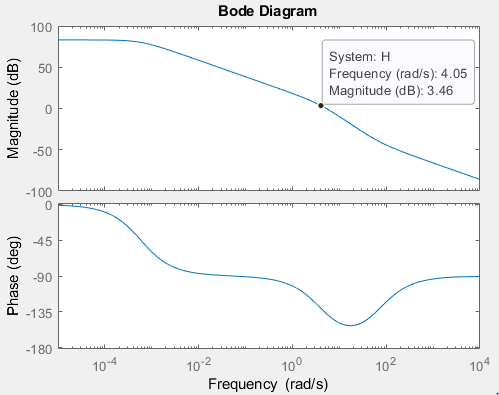
\includegraphics[width = 1.1\linewidth]{src/tex/img/bode.PNG}
\end{figure}
\end{column}
\begin{column}{0.4\textwidth}
\begin{itemize}
    \item Largura de Banda Bastante Limitada
\end{itemize}
\end{column}
\end{columns}
\end{frame}

\section{Projeto Controlador}
\subsection{Controle Proporcional}


\begin{frame}{LGR da planta no plano Z}
\begin{figure}
    \centering
    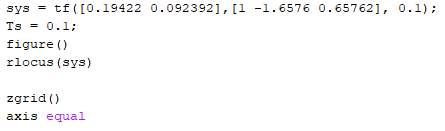
\includegraphics[width = \linewidth]{src/tex/img/script.PNG}
    \caption{}
    \label{fig:control_1}
\end{figure}
\end{frame}

\begin{frame}{LGR da planta no plano Z}
\begin{figure}
    \centering
    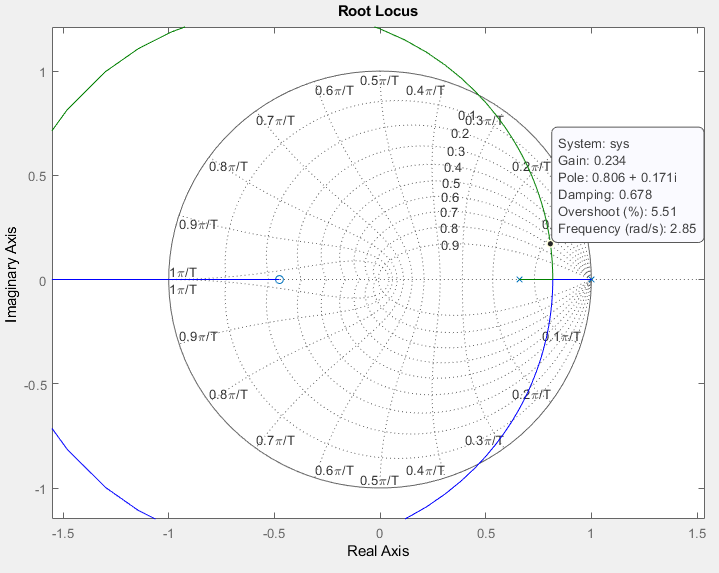
\includegraphics[width = 0.8 \linewidth]{src/tex/img/rlocus.PNG}
    \caption{}
    \label{fig:control_1}
\end{figure}
\end{frame}

\begin{frame}{Controle Proporcional}
\begin{figure}
    \centering
    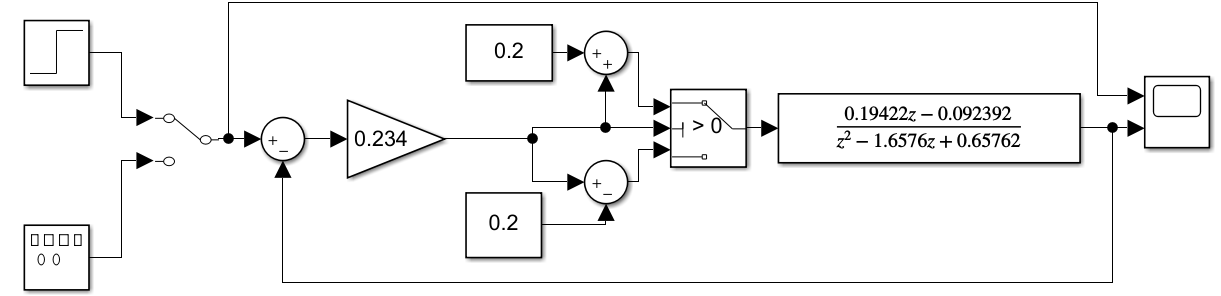
\includegraphics[width = \linewidth]{src/tex/img/controle_1.PNG}
    \caption{}
    \label{fig:control_1}
\end{figure}
\end{frame}




\begin{frame}{Resultados Controle Proporcional}
\begin{figure}
    \centering
    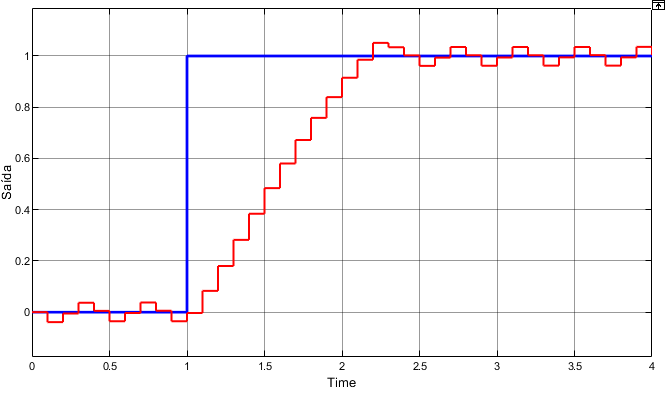
\includegraphics[width = \linewidth]{src/tex/img/saida_controle_1.png}
    \caption{}
    \label{fig:control_1}
\end{figure}
\end{frame}


\subsection{Projeto em Frequência}

\begin{frame}{Segunda proposta de Controlador}

Função de transferência da planta no domínio s:
\begin{equation}
G(s) = \frac{0.5011(s+70.0259)}{(s+0.00058419)(s+4.19042)}
\label{equacao_s}
\end{equation}

Estratégia: Anular o polo mais distante da planta e adicionar outro utilizando a equação de tempo de assentamento de uma sistema de segunda ordem:

\begin{equation}
\zeta \omega_{n}=\frac{4}{T_{s}}
\label{assentamento_eq}
\end{equation}

\begin{equation}
G_{c}(s)=\frac{s+4.19042}{s+8}
\label{novogc}
\end{equation}
\end{frame}

\begin{frame}{Segunda proposta de Controlador}

\begin{figure}[H]
    \centering
    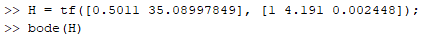
\includegraphics[width=0.7\linewidth]{src/tex/img/bode_comandos.PNG}
    \caption{Comandos no Matlab}
    \label{fig:lgr}
\end{figure}

\begin{figure}[H]
    \centering
    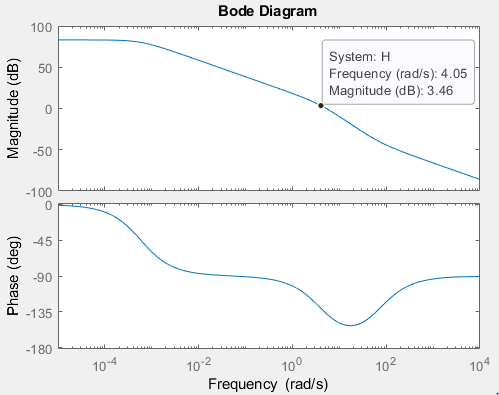
\includegraphics[width=0.6\linewidth]{src/tex/img/bode.PNG}
    \caption{Diagrama de bode}
    \label{fig:lgr}
\end{figure}

\end{frame}



\begin{frame}{Segunda proposta de Controlador}
Equação final do controlador:
\begin{equation}
G_{c}(z)=3.46\frac{s - 0.7116}{z - 0.4493}
\label{novogcz}
\end{equation}

\begin{figure}
    \centering
    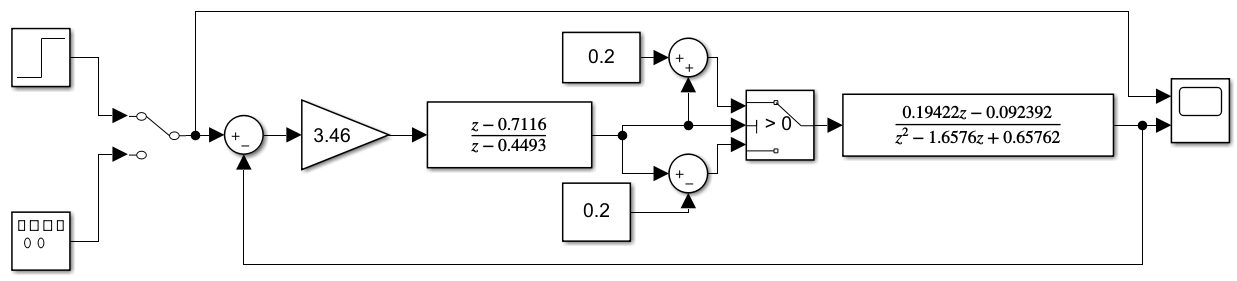
\includegraphics[width = \linewidth]{src/tex/img/controle_2.PNG}
    \caption{}
    \label{fig:control_2}
\end{figure}
\end{frame}

\begin{frame}{Resultados Segunda proposta de Controlador: Resposta ao degrau}
\begin{figure}
    \centering
    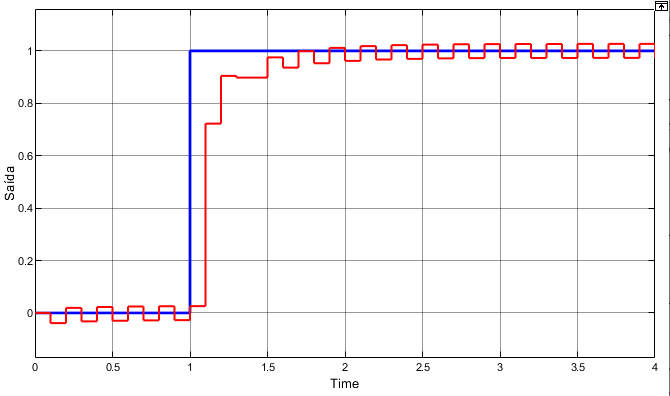
\includegraphics[width = \linewidth]{src/tex/img/saida_controle_2.png}
    \caption{}
    \label{fig:controler1}
\end{figure}
\end{frame}

\begin{frame}{Resultados Segunda proposta de Controlador: Resposta a onda quadrada}
\begin{figure}
    \centering
    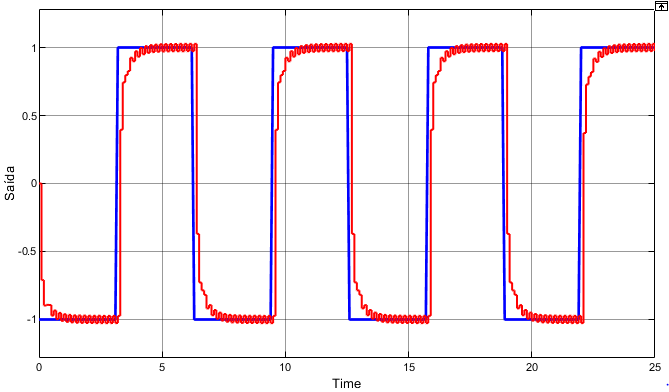
\includegraphics[width = \linewidth]{src/tex/img/teste_square.PNG}
    \caption{Resposta Controlador Atraso}
    \label{fig:controler2}
\end{figure}
\end{frame}

\begin{frame}{Resposta em Hardware ao primeiro controlador}
\begin{figure}
    \centering
    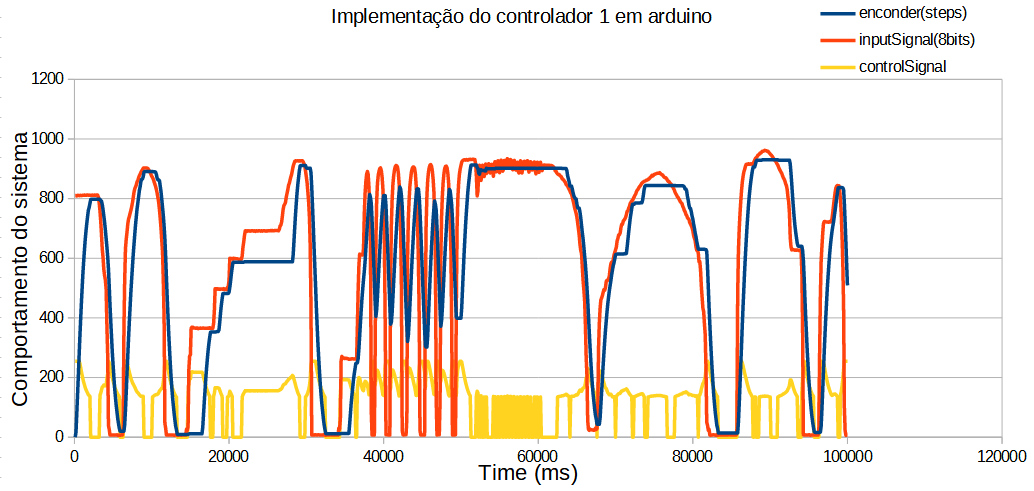
\includegraphics[width = \linewidth]{src/tex/img/resultado_controle_1_implem.PNG}
    \caption{Resposta Planta - $K_p = 0.25$}
    \label{fig:control_1}
\end{figure}
\end{frame}

\section{Conclusão}

\begin{frame}{Conclusão}
\begin{itemize}
    %\item Deu tudo errado
    \item O sistema final ficou lento
    \item Para variações lentas foi obtido um erro estacionário baixo
    \item Erro cumulativo da leitura de posição
    \item Controladores ajustados para a representação numérica
\end{itemize}
\end{frame}

\begin{frame}{Trabalhos Futuros}
% Modelagem Matemática
\begin{itemize}
    \item Implementação de filtros para o encoder
    \item Projeto controladores no espaço de estados
    \item Projeto PID completo
    \item Medir tempos usando hardware externo como forma de remover a necessidade da comunicação serial
    \item Calibrar as medidas do enconder com base em um sistema externo.
\end{itemize}
\end{frame}

\begin{frame}{}
% Obrigado!
\centering
\Huge{Obrigado!}
\end{frame}

\nocite{nise2012}

\begin{frame}{Referências}
\bibliographystyle{abbrv} % Define Estilo e gera bibliografia
\bibliography{references} % Adiciona Arquivo com Referências
\end{frame}


\end{document}